\newpage
\section{Feedback in Text Retrieval}

Feedback = learn from examples

\subsection{Types of Feedback}
\begin{itemize}
\item Relevance Feedback \\ Users make explicit relevance judgments on the initial results. Judgments are reliable, but users don’t want to make extra effort.
\item Pseudo/Blind/Automatic Feedback. \\ Top-k initial results are simply assumed to be relevant. Judgments aren’t reliable, but no user activity is required.
\item Implicit Feedback. \\ User-clicked docs are assumed to be relevant; skipped ones non-relevant. Judgments aren’t completely reliable, but no extra effort from users.
\end{itemize}


%----------------------------------------------
\subsection{Feedback in Vector Space Model}

How can a TR system learn from examples to improve retrieval accuracy? General method - query modification:
\begin{itemize}
\item Adding new (weighted) terms (query expansion)
\item Adjusting weights of old terms
\end{itemize}


%----------------------------------------------
\subsubsection{Rocchio Feedback}
\begin{figure}[H]
    \centering
    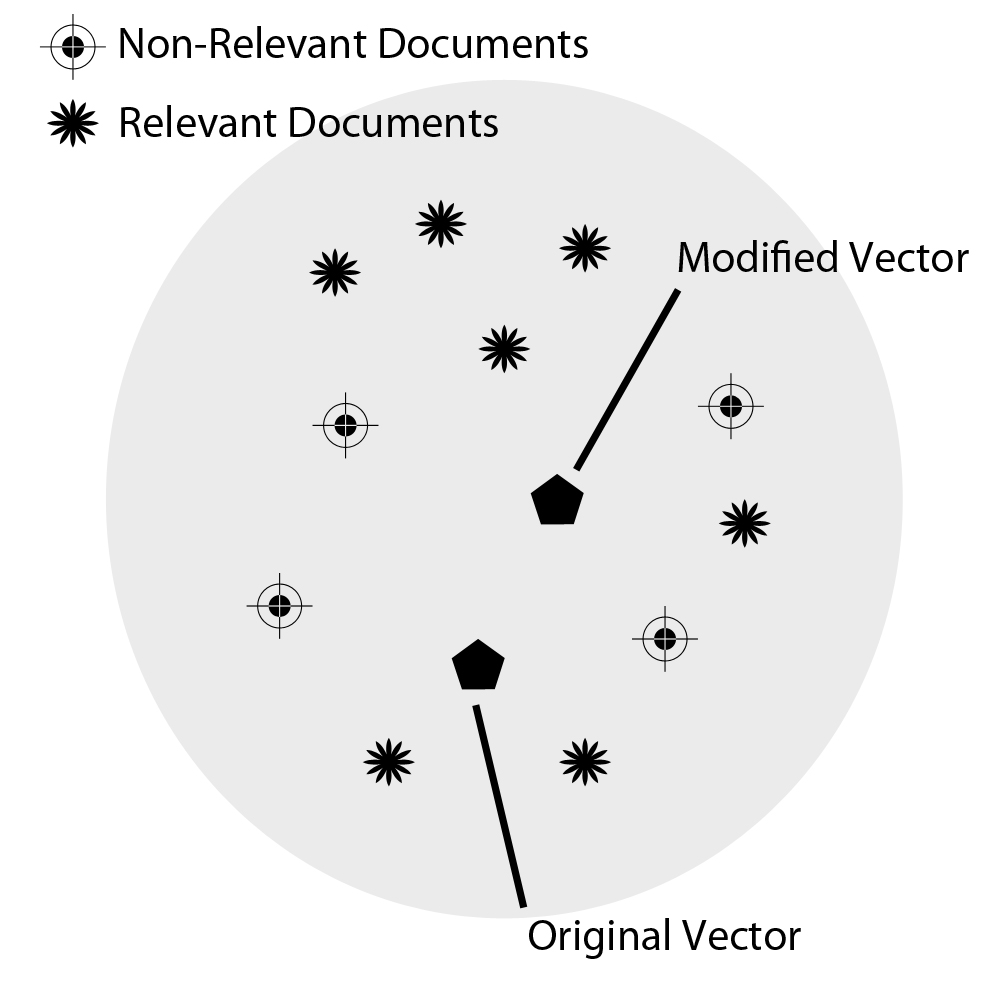
\includegraphics[width=0.6\linewidth]{Rocchio.jpg}
\end{figure}

\begin{equation*}
\overrightarrow{Q_m} = \bigl(\alpha \cdot \overrightarrow{Q_o} \bigr) + \biggl( \frac{\beta}{|D_r|} \cdot \sum_{\overrightarrow{D_j} \in D_r} \overrightarrow{D_j} \biggr)
- \biggl(\frac{\gamma}{|D_{nr}|} \cdot \sum_{\overrightarrow{D_k} \in D_{nr}} \overrightarrow{D_k} \biggr) 
\end{equation*}

\begin{itemize}
\item $\overrightarrow{Q_m}$ - Modified Query Vector
\item $\overrightarrow{Q_o}$ - Original Query Vector
\item $\overrightarrow{D_j}$ - Related Document Vector
\item $\overrightarrow{D_k}$ - Non-Related Document Vector
\item $\alpha$ - Original Query Weight
\item $\beta$ - Related Documents Weight
\item $\gamma$ - Non-Related Documents Weight
\item $D_r$ - Set of Related Documents
\item $D_{nr}$ - Set of Non-Related Documents
\end{itemize}

%----------------------------------------------
\subsubsection{Rocchio in Practice}
\begin{itemize}
\item Negative (non-relevant) examples are not very important
\item Often truncate the vector (i.e., consider only a small number of words that have highest weights in the centroid vector) (efficiency concern)
\item Avoid <<over-fitting>> (keep relatively high weight on the original query weights)
\item Can be used for relevance feedback and pseudo feedback ($\beta$ should be set to a larger value for relevance feedback than for pseudo feedback)
\item Usually robust and effective
\end{itemize}


%----------------------------------------------
\subsection{Feedback in Language Model}

\subsubsection{The KL-divergence measure}
Given two probability mass functions $p(x)$ and $q(x)$, the Kullback-Leibler divergence (or relative entropy) between $p$ and $q$ is defined as:
\begin{equation*}
D(p \parallel q) = \sum_x p(x) \log \frac{p(x)}{q(x)}
\end{equation*}

%--------------
\subsubsection{Kullback-Leibler (KL) Divergence Retrieval Model}

KL-divergence (cross entropy):
\begin{equation*}
f(q, d) = \sum_{\substack{w \in d, \\ p(w \mid \hat{\theta}_Q)>0}} p(w \,\big|\, \hat{\theta}_Q) \log \frac{p_{seen}(w_i \,\big|\, d)}{\alpha_d \, p(w_i \,\big|\, \mathcal{C})} + \log \alpha_d
\end{equation*}
\begin{itemize}
\item $\hat{\theta}_Q$ - estimated query unigram language model
\end{itemize}


If query language model is maximum likelihood $p_{ml}(w \,\big|\, \hat{\theta}_Q) = \dfrac{c(w, q)}{|q|}$, then KL-divergence becomes a query likelihood retrieval formula:
\begin{equation*}
f(q, d) = \sum_{\substack{w_i \in d, \\ w_i \in q}} c(w_i, q) \log \frac{p_{seen}(w_i \,\big|\, d)}{\alpha_d \, p(w_i \,\big|\, \mathcal{C})} + n \log \alpha_d
\end{equation*}

%--------------
\subsubsection{Feedback as Model Interpolation}
\begin{figure}[H]
    \centering
    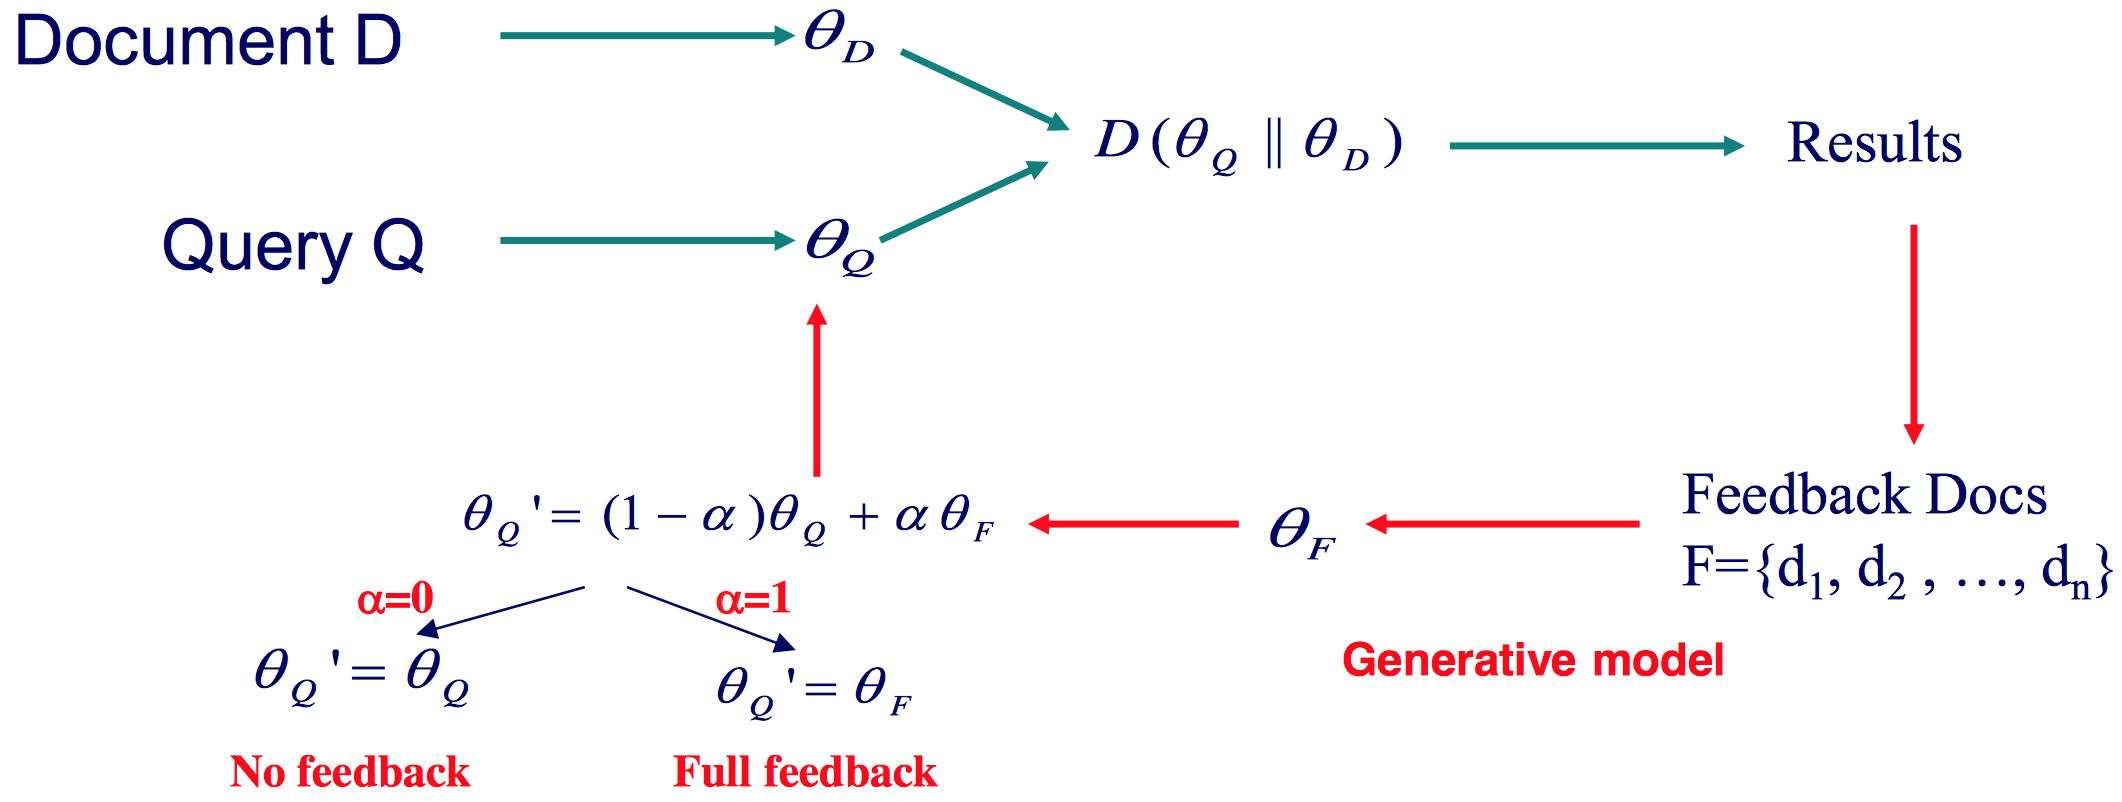
\includegraphics[width=0.8\linewidth]{LM_feedback.png}
\end{figure}

\begin{equation*}
p(w \,\big|\, \hat{\theta}_Q) = (1-\alpha) \, p_{ml}(w \,\big|\, \hat{\theta}_Q) + \alpha \, p(w \,\big|\, \theta_F)
\end{equation*}
\begin{itemize}
\item $\alpha$ is a parameter that needs to be set empirically
\item $p(w \,\big|\, \theta_F)$ is a feedback model
\end{itemize}

%--------------
\subsubsection{Generative Mixture Model}
\begin{figure}[H]
    \centering
    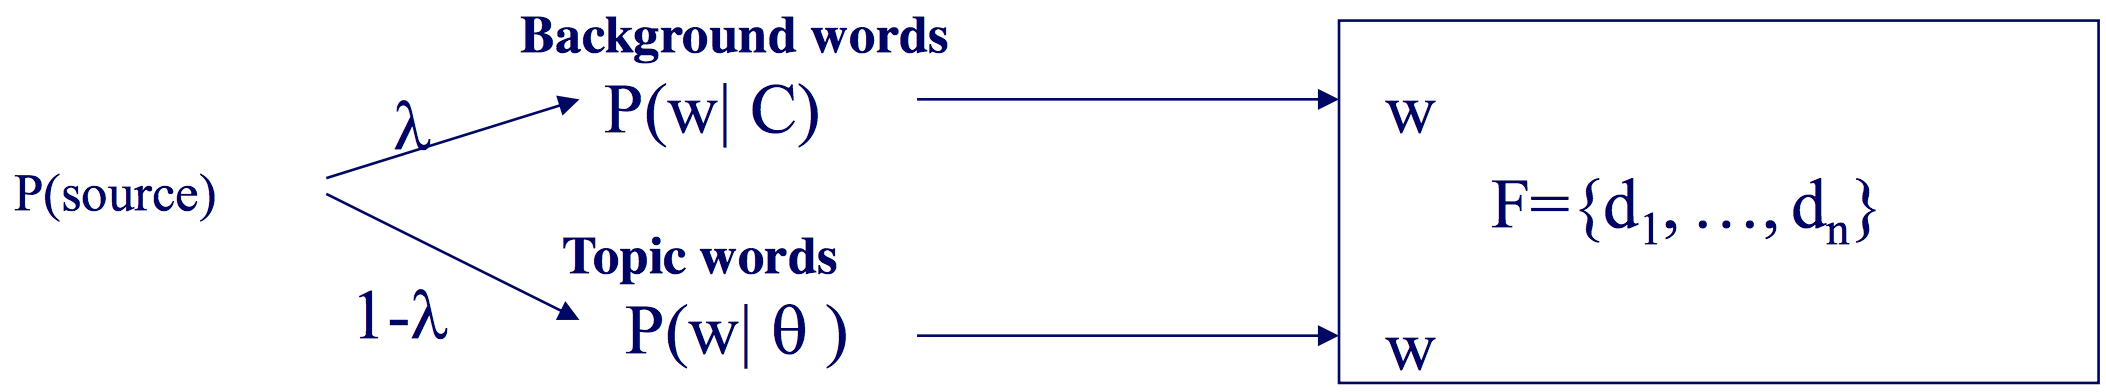
\includegraphics[width=0.8\linewidth]{mixture_model.png}
\end{figure}

\begin{equation*}
\log p(\mathcal{F} \,\big|\, \theta_F) = \sum_{i=1}^n \sum_w c(w, d_i) \log \left( (1-\lambda) p(w \,\big|\, \theta_F) + \lambda p(w \,\big|\, \mathcal{C}) \right)
\end{equation*}
\begin{itemize}
\item $F = \{d_1, \dots , d_n \}$ - the set of feedback documents
\item $\lambda$ - parameter that indicates the amount of <<background noise>> in the feedback documents
\end{itemize}

Maximum likelihood estimate of $\hat{\theta}_F$:
\begin{equation*}
\hat{\theta}_F = \argmax_{\theta_F} \, \log p(\mathcal{F} \,\big|\, \theta_F)
\end{equation*}


%----------------------------------------
\subsection{Recommended reading}
\begin{itemize}
\item ChengXiang Zhai, \href{http://www.morganclaypool.com/doi/abs/10.2200/S00158ED1V01Y200811HLT001}{<<Statistical Language Models for Information Retrieval>> (Synthesis Lectures Series on Human Language Technologies)}, Morgan \& Claypool Publishers, 2008.
\item Victor Lavrenko and W. Bruce Croft. 2001. <<Relevance based language models>>. In Proceedings of ACM SIGIR 2011. 
\end{itemize}

